
\begin{supplementary}

\section{Supporting Information}

\subsection{"dFBA" module}
We attempted to repurpose the "dFBA" module into a scalable and more accessible module for Windows OS. This was inhibited by the “dfba\_utils.so” file, and our attempt to replace this file with a dynamic linked library (DLL) analogue was thwarted by incompatibilities between C code in the library dependencies such as NVectors, SUNDIALS, and dlfcn and the C++ code of the DLL file. A further complication was that a few of these libraries, such as SUNDIALS, dynamically created the header files depending upon the user’s operating system; thus, a distinct DLL file would be required for each possible user architecture, which is not practical. The dFBApy module was therefore developed. 

\subsection{Thermodynamic metabolism}
We considered conducting metabolism for WCMpy via thermodynamic gradients, rather than conventional dFBA kinetics. This proposed logic is incomplete, since we migrated to the kinetic models during its development; however, the preliminary logic and calculations of the following sub-sections may still inspire the development of a thermodynamic metabolic approach.  

\subsubsection{Membrane absorption}

\begin{figure}
    \centering
    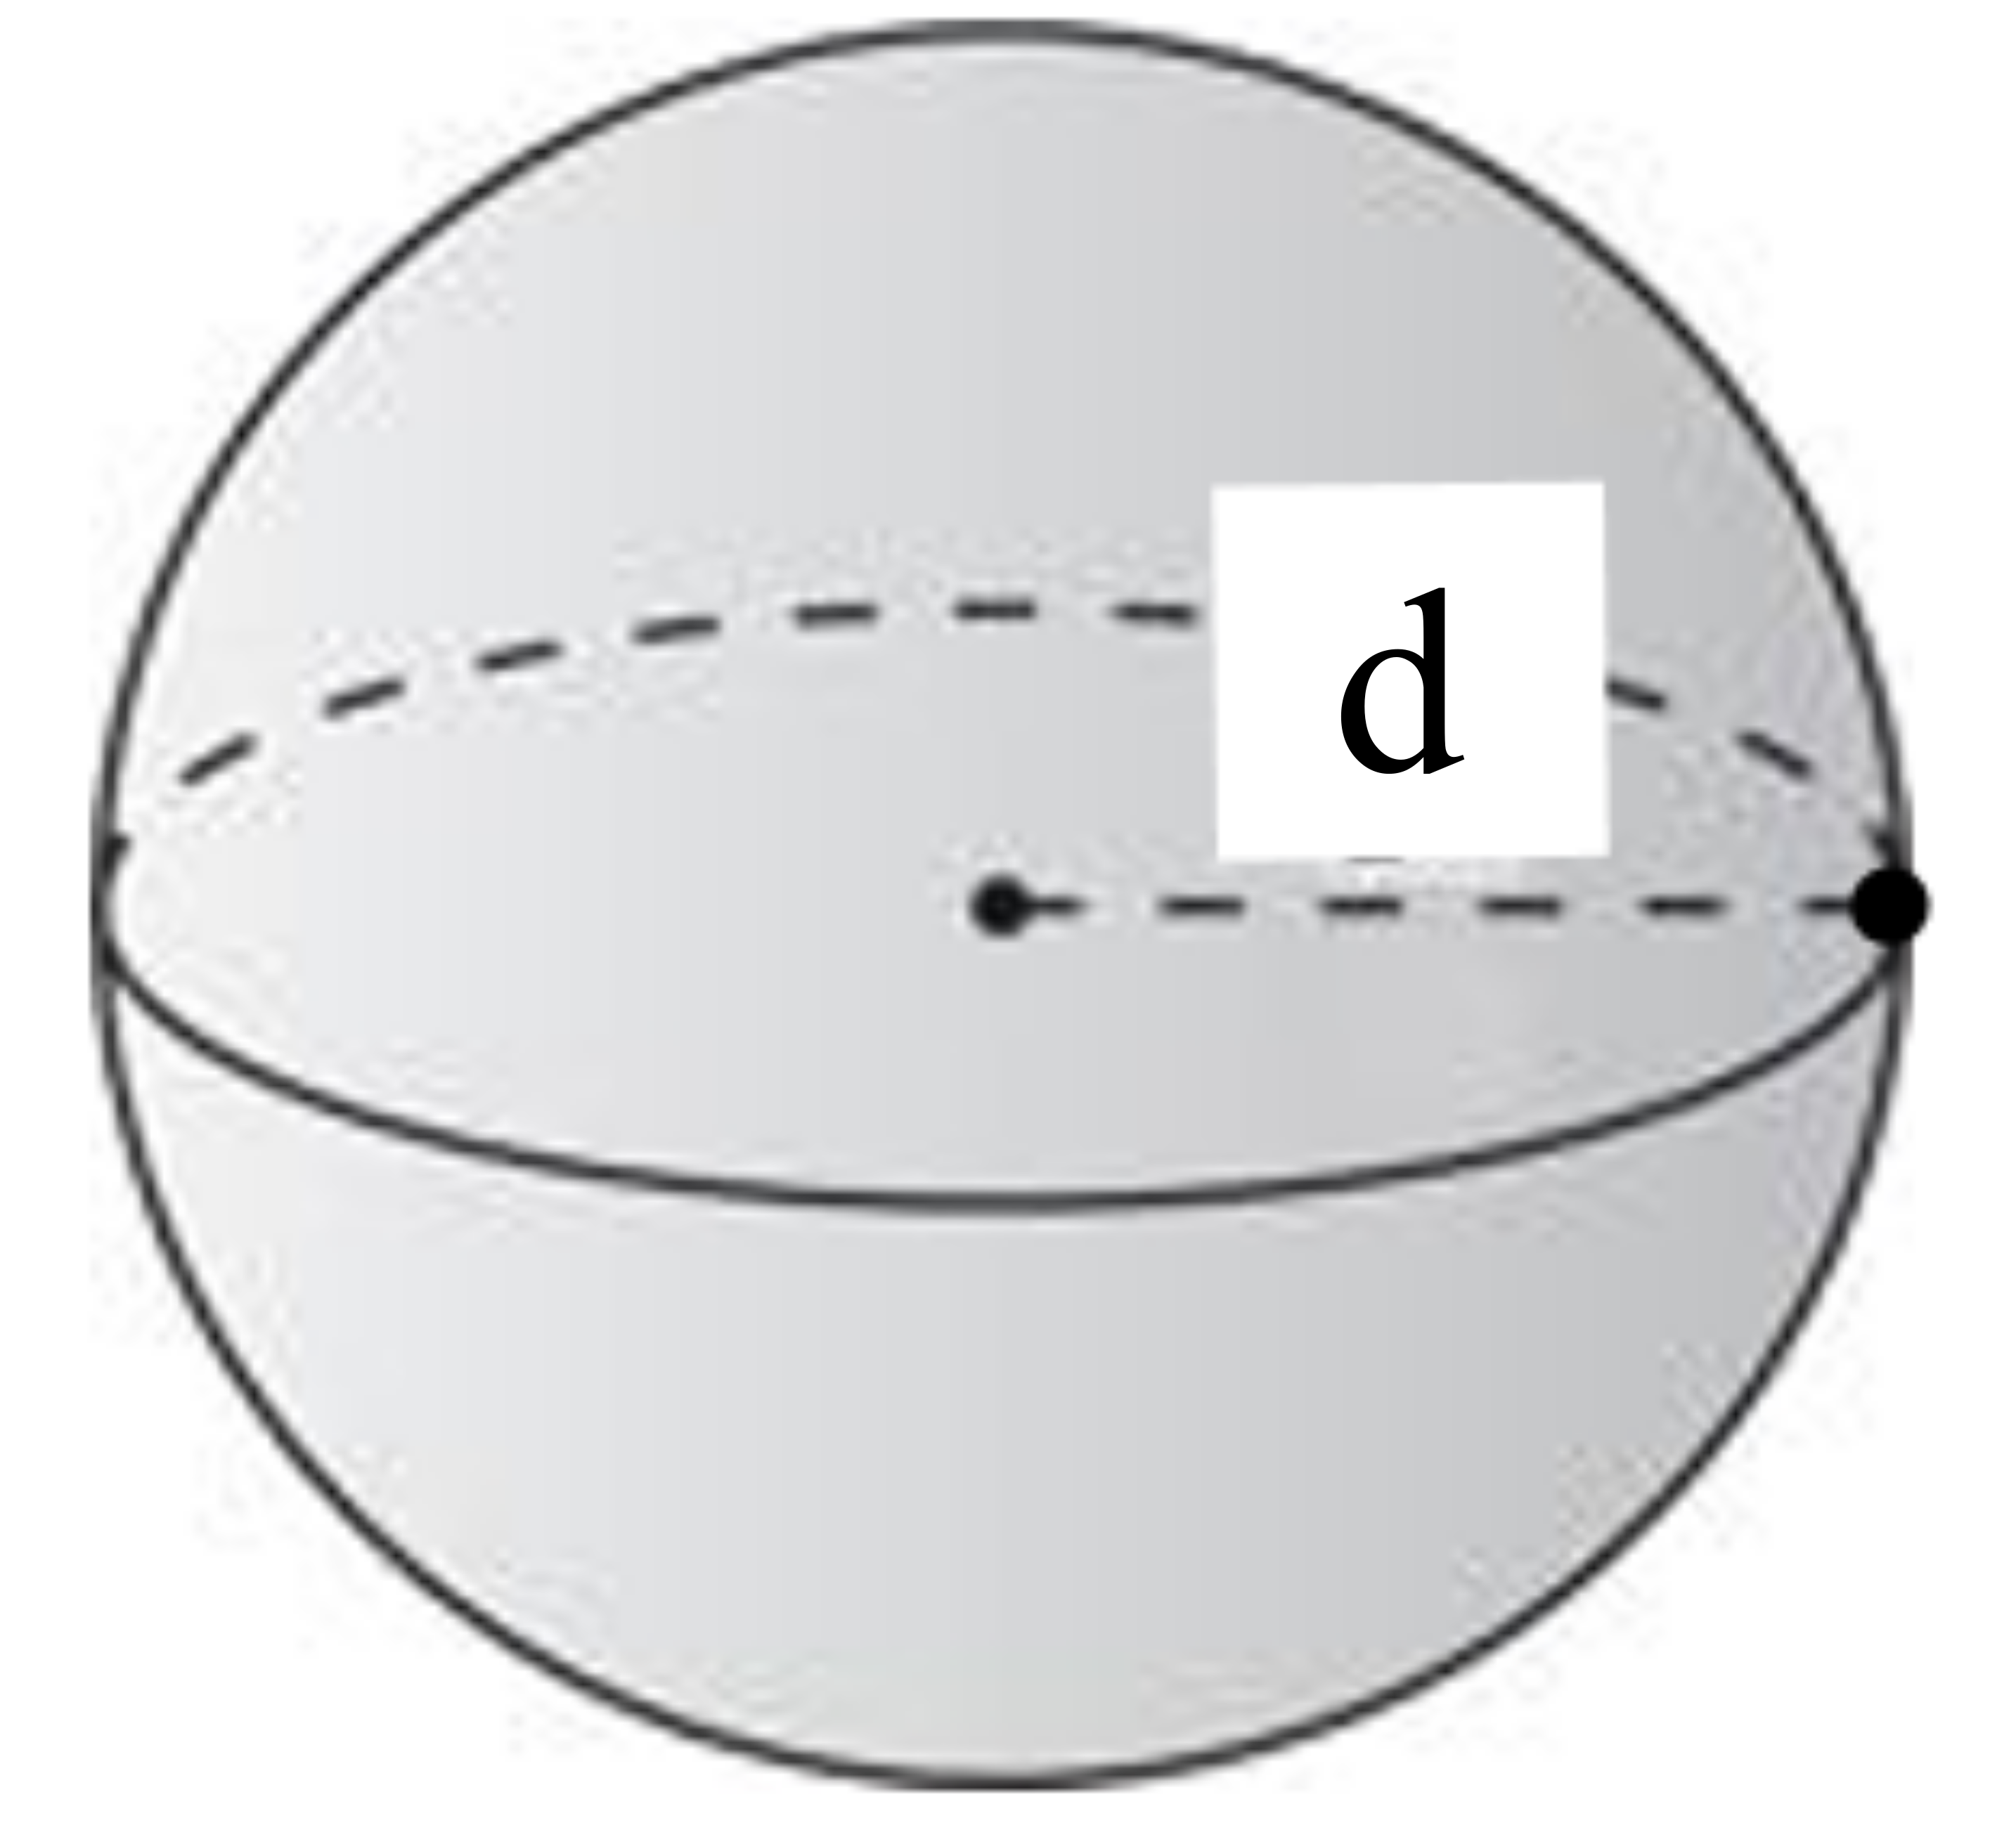
\includegraphics[width = 0.5\textwidth]{images/WCMpy/diffusion_sphere.png}
    \caption{
        A sphere where the surface area represents the location of a chemical after a timestep, which begins at the origin of the sphere, while possessing the average root-mean-squared velocity of extracellular chemicals.
    }
    \label{diffusion_sphere}
\end{figure}

\begin{figure}
    \centering
    \begin{subfigure}[b]{0.46\textwidth}
        \centering
        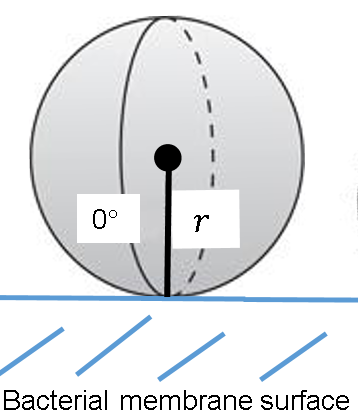
\includegraphics[width = \textwidth]{images/WCMpy/maximal_far.png}
        \caption{
            The maximal distance (d) from the bacterial membrane where a chemical can still contact the membrane with a timestep. This distance defines the thickness of the volume shell around the bacterial membrane within which chemicals may potentially be absorbed in a timestep.   
        }
    \end{subfigure}
    \hfill
    \begin{subfigure}[b]{0.47\textwidth}
        \centering
        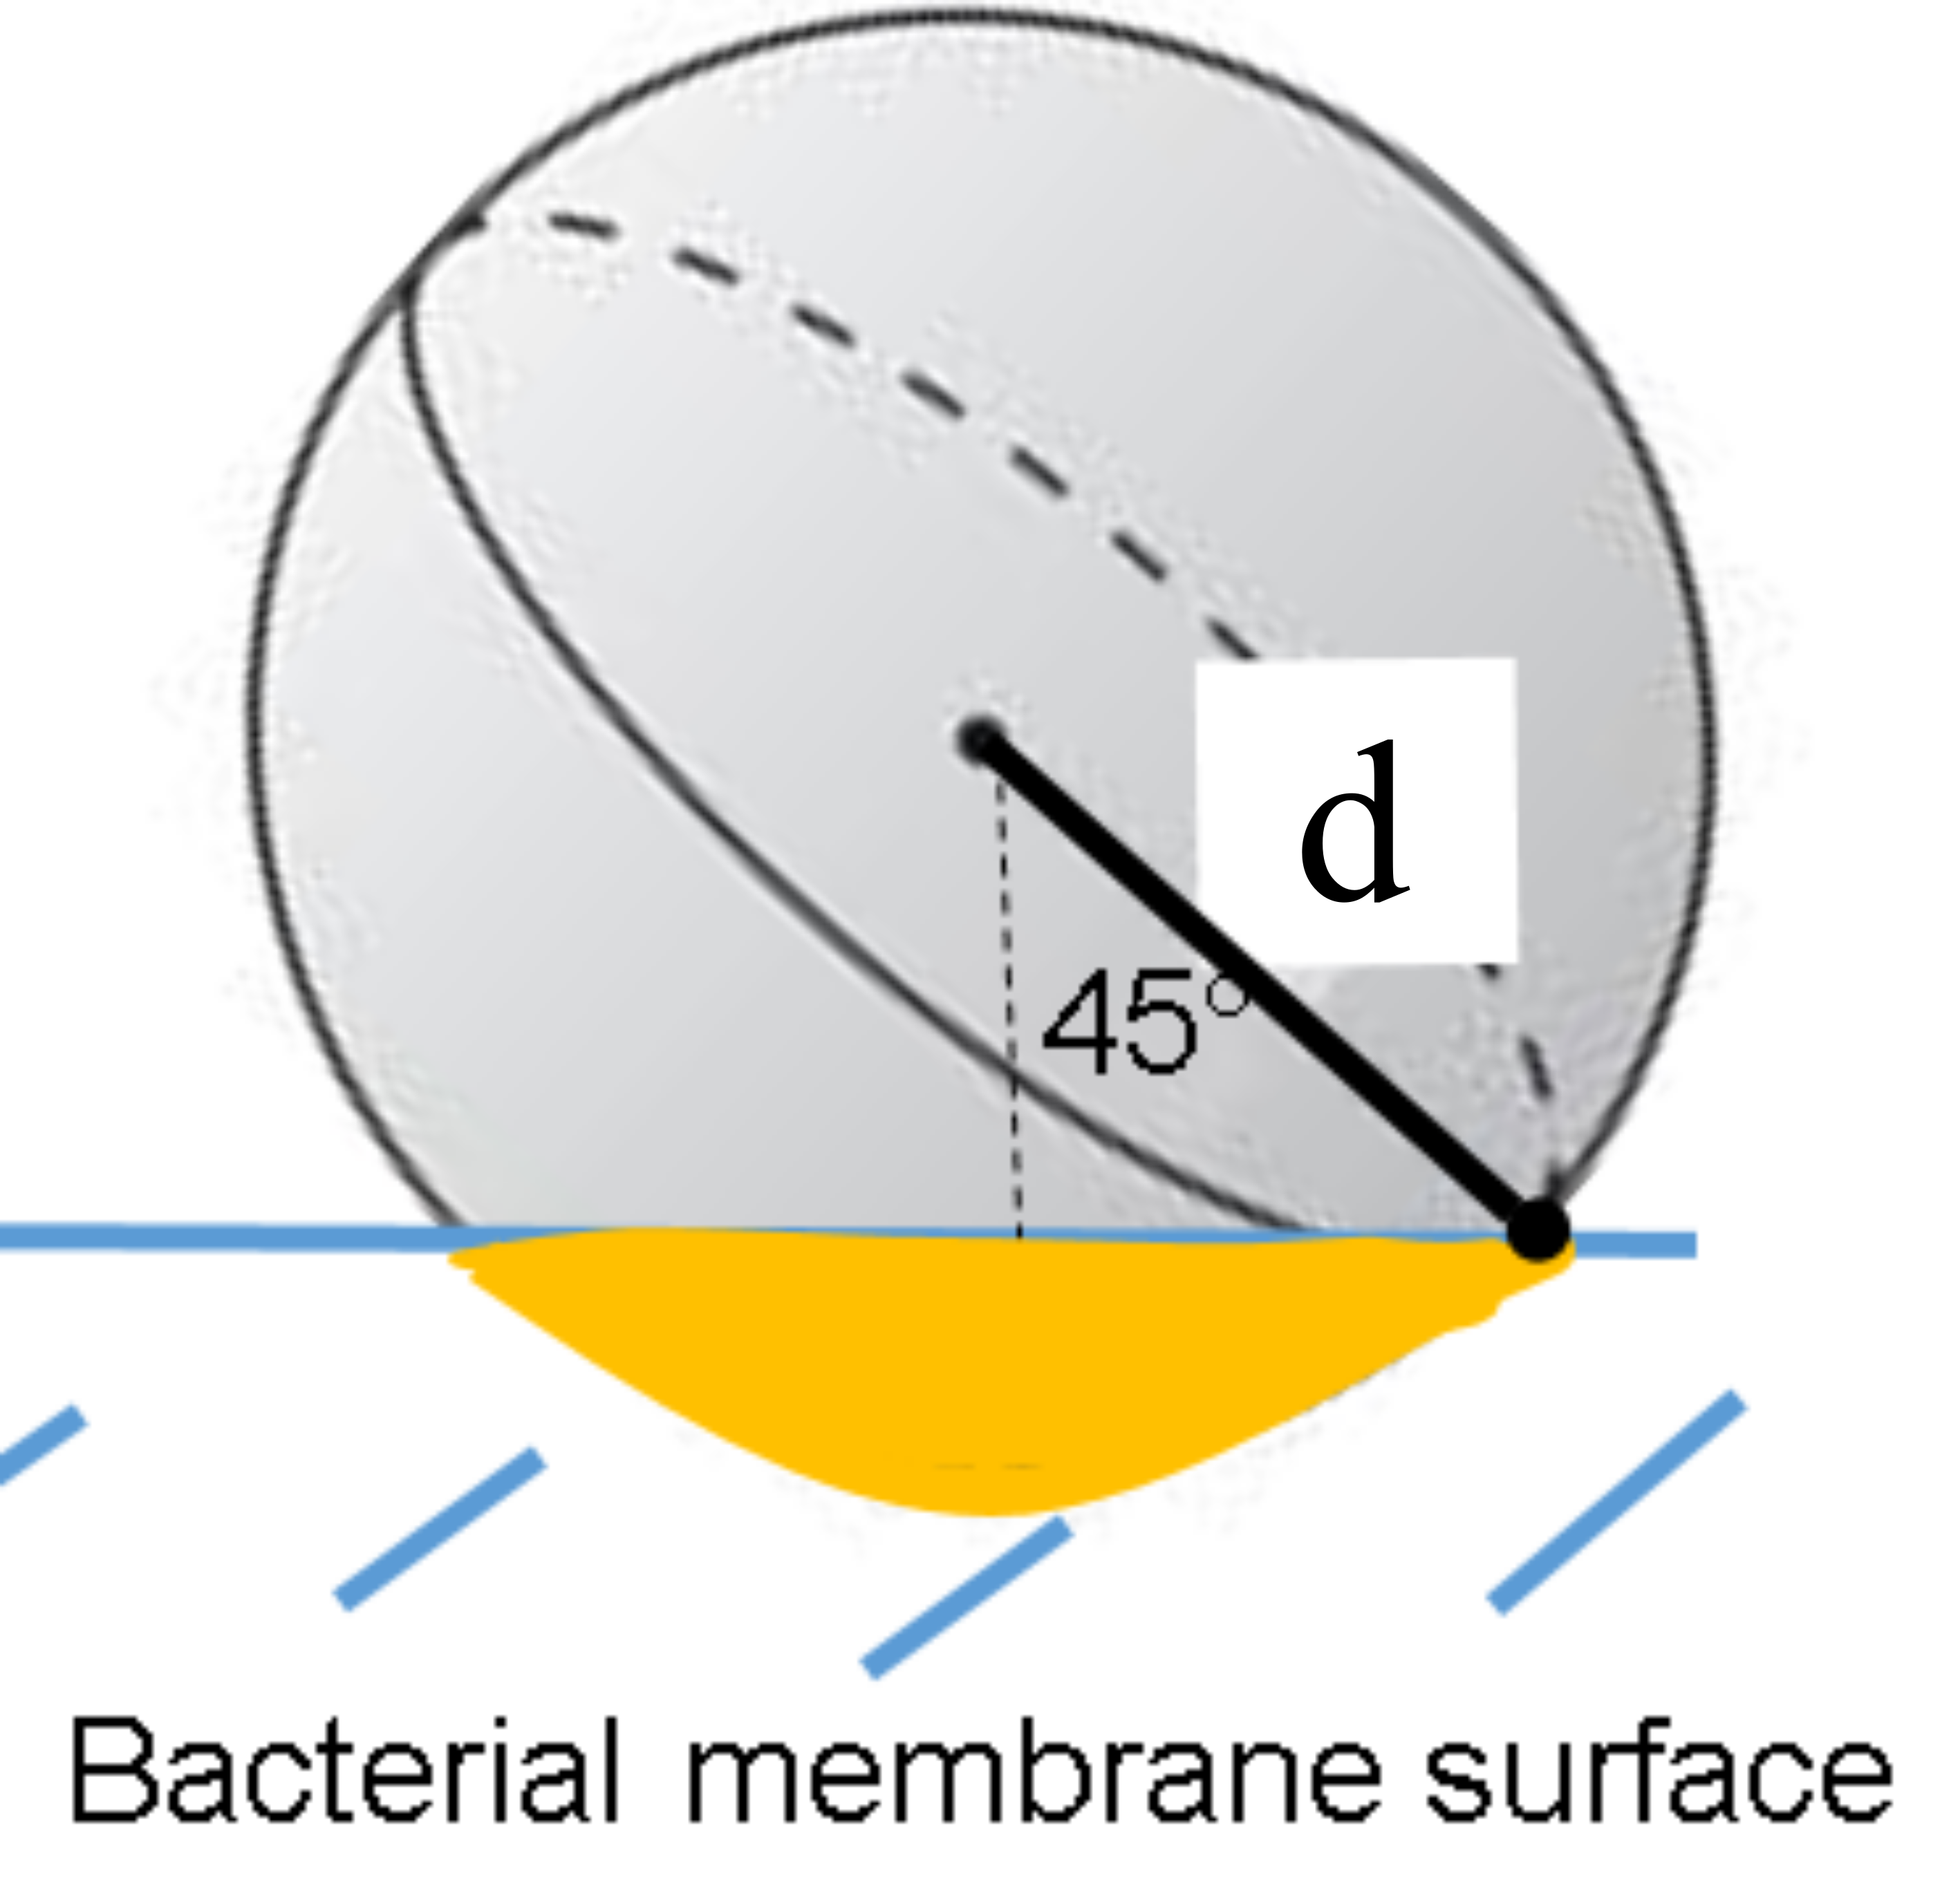
\includegraphics[width = \textwidth]{images/WCMpy/average_far.png}
        \caption{
            The average distance ($d*cos(45\degree)$) from the bacterial membrane where a chemical can still contact the membrane with a timestep. The proportion of the orange surface area and the total surface area in \cref{collision_probability} represents the probability of that a chemical within the volume shell around bacterial membrane strikes the membrane in a timestep.
        }
    \end{subfigure}
    \caption{
          Distances from the bacterial membrane where an extracellular chemical can still contact the membrane within the timestep, given a known velocity.
    }
    \label{diffusion_distances}
\end{figure}

Cellular absorption is determined by the cellular dimensions, which are calculated with each timestep. The bacterial shape is assumed to be spherical, which facilitates calculating cellular volume and surface area as a function of cellular mass $m$, via a constant density, with each timestep $\Delta t$. The quantity of absorbed chemicals is calculated as a fraction of the chemicals that exist within a distance $d$ from the bacterial membrane,
\begin{equation}
    d=\overset{\rightharpoonup}{V}_{rms}*\Delta t~.
\end{equation} 
This is the distance that a chemical, with the average root-mean-squared velocity of an extracellular chemical
\begin{equation}
    \overset{\rightharpoonup}{V}_{rms}=\sqrt{\frac{3*k_B*T}{m_{ave}}}~,
\end{equation} 		
travels in $\Delta t$, where $k_B$ is the Boltzmann constant; $T$ is the extracellular temperature in kelvins; and $m_{ave}$ is the average mass of the extracellular chemicals. The distribution of potential locations for a chemical after $\Delta t$ is conceptually represented as a sphere in Figure \ref{diffusion_sphere}, where the origin is the initial location of the chemical and the sphere surface, a $d$ distance from its origin, represents the set of possible final locations. The volumetric shell of $d$ thickness around the bacterial membrane is the volume wherein chemicals could potentially collide with the membrane and be absorbed, which is calculated
\begin{equation} \label{shell_volume}
    V_{shell}=\frac{4\pi}{3}*((r_{cell}+d)^3-r_{cell}^3)
\end{equation}
where $r_{cell}$ is the cellular radius at the start of $\Delta t$. The product of $V_{shell}$ and the extracellular chemical concentration $C_i$ of chemical $i$ 
\begin{equation} \label{shell_quantity}
    n_{shell,i}=C_i*V_{shell}
\end{equation}
yields the $n_{shell,i}$ quantity of chemical $i$ that may be potentially absorbed. The proportion $P$ of $n_{shell,i}$ that will contact the membrane is calculated as the proportion of spherical surface area in Figure \ref{diffusion_distances}b that overlaps with the membrane
\begin{equation} \label{collision_probability}
    P = \frac{SA_{membrane~collisions}}{SA_{sphere~of~possibilities}} = \frac{
    2*\pi*r_{distance~traveled}*(r_{distance~traveled}*cos(contact\_angle))
    }{
    4*\pi*r_{distance~traveled}^2
    } = \frac{(cos(45\degree))}{2} = 14.6\%~.
\end{equation}
The numerator is mathematically represented as the surface area of a conic sector of the chemical location sphere. The $contact\_angle$ of $45\degree$, between the extracellular chemical and the bacterial membrane, is the average between the maximal angle of $90\degree$ for the infinitesimally close chemical to the membrane and the minimal angle of $0\degree$ for the farthest possible chemical, which is illustrated in Figure \ref{diffusion_distances}a. The $P$ value of \cref{collision_probability} is importantly independent and constant. 

The fraction of incident $P$ chemicals that are absorbed is approximated by the thermodynamic gradient of each chemical $i$, which we propose represents the metabolic need $E_i$ of that chemical. The thermodynamic gradient is determined as the current displacement $\Pi_{R=1}^x (\frac{Q_R}{K_{eq, R}})$ -- for the $x$ number of $R$ reactions in which chemical $i$ is a reactant  -- from the optimum displacement 
\begin{equation}
    \left(\frac{Q}{K_{eq}}\right)_{optimum,i}=e^{\dfrac{\eta*n_{e^-,i}* F * E_{potential}}{R*T_{incubation}}}
\end{equation}
where $\eta$ is the total quantity of reactions in the bacterial membrane; $n_{e^-,i}$ is the average quantity of exchanged electrons in reactions where chemical $i$ is a reactant; $F$ is Faraday’s constant of electrical charge; $E_{potential}$ is the electrical potential of the bacterial membrane; $R$ is the gas constant; and $T_{incubation}$ is the incubation temperature of the simulated organism, which we presume to be indicative of the optimal thermodynamic displacement for the organism's biochemistry. The metabolic need
\begin{equation} \label{metabolic_need}
    E_i= \begin{cases}
            0, ~~\text{if} \left(\frac{Q}{K_{eq}}\right)_{optimum,i}<\Pi_{R=1}^x \left(\frac{Q_R}{K_{eq, R}}\right) \\
            \left(\frac{Q}{K_{eq}}\right)_{optimum,i}-\Pi_{R=1}^x \left(\frac{Q_R}{K_{eq, R}}\right), ~~\text{else}
        \end{cases} 
\end{equation}
is constrained to be positive, which assumes that excessive chemicals are not jettison. The absorbed quantity of chemical $i$
\begin{equation}
    n_{absorbed,i}=E_i*n_i*P*B_i~,
\end{equation}
is finally the product of its metabolic need ($E_i$ from \cref{metabolic_need}), its quantity within the volume shell ($n_i$ from \cref{shell_volume,shell_quantity}), the probability of it striking the membrane ($P$ from \cref{collision_probability}), and finally absorption hindrances that are encapsulated in $B_i$ to abstractly represent transport phenomena at the membrane that may discriminately treat different chemicals. The contribution of absorption to mass growth of the cell is calculated
\begin{equation} \label{mass_change}
    \frac{\Delta m}{\Delta t}=\sum_{i=1}^b(n_{absorbed,i}*MW_i-n_{ejected~waste,i}*MW_i)
\end{equation}
as the sum-product of the quantity of all absorbed or disposed $b$ chemicals in the metabolism and their respective molecular weights. The aggregate change in the cellular mass $\frac{\Delta m}{\Delta t}$ from \cref{mass_change} begets cellular dimensions
\begin{equation}
    r_{cell}=\left(\frac{3*\frac{m}{\delta_{cell}}}{4*\pi}\right)^{\dfrac{1}{3}}~,
\end{equation}
assuming a constant density ($\delta_{cell}$). 


\subsubsection{Chemical reactions}

Metabolic reactions are partitioned between the cytoplasm (c), the membrane (m), and the extracellular environment (e). The maximal possible quantity of chemical reactions that can proceed in the forward or backward directions is calculated $R_{max}=\left|\frac{C_i}{s}\right|$, where $C_i$ is the concentration of chemical $i$ and $s$ is the stoichiometry of chemical $i$ in reaction $R$. The maximal $R_{max}$ reaction progressions in a $\Delta t$ is attenuated $R_{actual}=R_{max}*\zeta$ by a scalar $\zeta$ that represents unreactive collisions and diffusion limitations \cite{Feynman1963ChapterDiffusion}. The $R_{actual}$ is further limited $R_{actual} = \begin{cases} R_{actual},~~if~R_{actual}<e \\ e,~~else \end{cases}$ by the quantity of enzymes that can catalyze the reaction \textit{e}. The direction of the $R_{actual}$ reactions is determined $NF = K_{eq}-Q$ by the relative difference between the current $Q$ and optimal $K_{eq}$ thermodynamic values, where $NF>0$ denotes forward reactions and $NF<0$ denotes backward reactions. The concentration change $C_i$ -- in each separate compartment -- over the timestep for chemical $i$ is calculated $\frac{dC_i}{dt}=R_{actual}*s$ as the product of the quantity of reaction progressions and the respective stoichiometry of the chemical in the reaction. The new $C_i$ is crucially used in \cref{metabolic_need} to determine the metabolic need of the chemical in the system. 

\end{supplementary}